
Um den Effekt der nebenläufigen Architektur möglichst zu isolieren, werden in den Szenarien 1 und 2 keine zufällig generierten Welten genutzt. Stattdessen werden die Blöcke nach einem festgelegten Muster gesetzt.

\begin{figure}
	\centering
	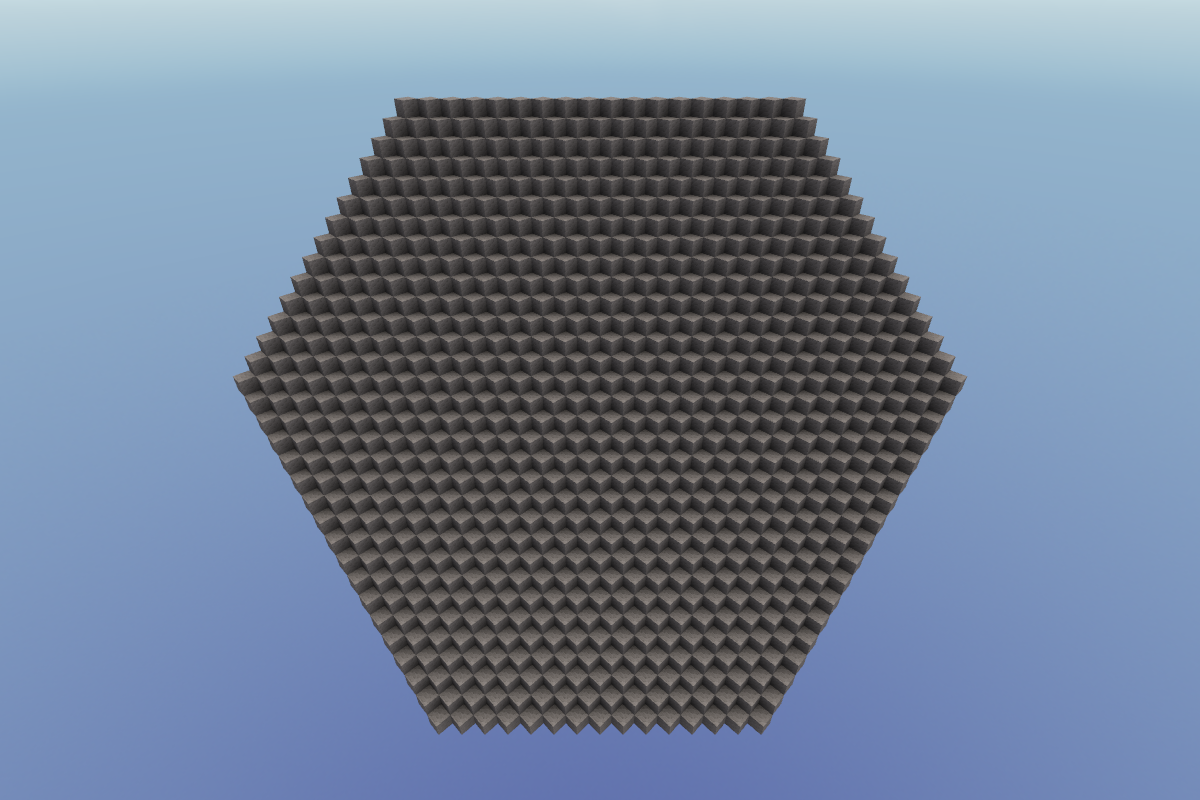
\includegraphics[width=.8\textwidth]{fps-hexagon.png}
	\caption[Screenshot der Blockformation in Szenario 1 der Performanceanalyse.]{Screenshot der Blockformation in Szenario 1. Die Blöcke bilden ein stilisiertes Hexagon. Es ist \emph{nicht} gleichseitig. Die Formation ermöglicht den Blick auf je drei Seiten jedes Blocks und besteht aus 766 Blöcken.}\label{fig:hexagon}
\end{figure}
Die Anordnung der Blöcke in Szenario 1 ist in Abbildung~\vref{fig:hexagon} dargestellt. Wie auf der Abbildung bei genauem Hinsehen zu erkennen ist, sind von jedem Block drei Seiten sichtbar. Dadurch lässt sich die genaue Anzahl der Elemente bestimmen, die gezeichnet werden. Damit lässt sich die Gesamtzahl der gezeichneten Polygone\footnote{In der Blocklib besteht jedes gezeichnete Element aus Dreiecken oder aus Rechtecken, zusammenfassend werden diese als Polygone bezeichnet. Die meisten Elemente in der Welt werden als Dreiecke gezeichnet, die Elemente der graphischen Oberfläche nutzen Rechtecke. Jede Seite eines Blocks aus zwei Dreiecken hier aus zwei Dreiecken zusammengesetzt. Siehe dazu auch Abbildung~\vref{fig:cube}.} für dieses Szenario genau berechnen. Jeden Frame müssen genau $766\cdot3\cdot2 + 3\cdot2-1 = 4596 +5 = 4601$ Polygone gezeichnet werden. Die $5$ zusätzlichen Polygone stammen von der \emph{Skybox}, einem großen Würfel um die Spielwelt herum, der eine Himmelstextur zeigt. Eines der Dreiecke der drei Seiten der Skybox ist außerhalb des Sichtfelds. Daher müssen nur $5$ Polygone hinzugezählt werden.

\begin{figure}[!htbp]
	\settowidth\mytemp{1,}
	\fpsplot[ytick={0,200,...,1200},height=5cm,ymax=1200,y label style={at={(ticklabel cs:.5,-\mytemp)}}]{seed-0-hexagon}
	\caption[Graph des Verlaufs der Framerate in Szenario 1: Hexagon.]{Graph des Verlaufs der Framerate im Szenario 1: Hexagon.}\label{fig:seed-0-hexagon-fps}
\end{figure}
\paragraph{\ac{fps}} Abbildung~\vref{fig:seed-0-hexagon-fps} zeigt den Verlauf der \si{\fps}. Die Framerate unter SystemA ist durchschnittlich \SI{337}{\fps} unter SystemB \SI{1133}{\fps}. Das ist ein Zuwachs von \SI{236}{\percent}. Unter SystemA ist der Start der Blocklib schneller. Hier werden Frames nach \SI{11,2}{\second} erzeugt, in SystemB nach \SI{13,6}{\second}. SystemB benötigt für den Start also \SI{21}{\percent} mehr Zeit. Über die Zeit hinweg bleiben die Frameraten beider Systeme in etwa konstant.


\begin{figure}[!htbp]
	\cpuplot{seed-0-hexagon}
	\caption{Seed 0 Hexagon}\label{fig:seed-0-hexagon-cpu}
\end{figure}
\paragraph{\ac{cpu}} Der Verlauf der Auslastung der \ac{cpu} durch die Blocklib ist in Abbildung~\vref{fig:seed-0-hexagon-cpu} zu sehen. Beide Systeme zeigen hier eine Spitze in der Auslastung beim Start der Blocklib. In SystemA ist die maximale Auslastung von \SI{47}{\percent} nach \SI{11,6}{\second} erreicht, SystemB erreicht eine Auslastung von \SI{42}{\percent} nach \SI{15,6}{\second}. Die maximale Auslastung ist bei SystemB \SI{11}{\percent} niedriger als bei SystemA. Die durchschnittliche Auslastung in der Hauptphase ist in SystemB mit einem Wert von \SI{18}{\percent} um \SI{38}{\percent} höher als in SystemB mit durchschnittlich \SI{13}{\percent}. Nach den anfänglichen Spitzen ist die Auslastung in beiden Systemen in etwa konstant.

\begin{figure}[!htbp]
	\gpuplot{seed-0-hexagon}
	\caption{Seed 0 Hexagon}\label{fig:seed-0-hexagon-gpu}
\end{figure}
\paragraph{\ac{gpu}} Der in Abbildung~\vref{fig:seed-0-hexagon-gpu} dargestellte Graph beschreibt die Auslastung der \ac{gpu} im zeitlichen Verlauf. Da für diese Messungen ein externer Profiler genutzt wird, kann die Auslastung der \ac{gpu} über die gesamte Messdauer hinweg ermittelt werden. Die Daten zu Beginn und zum Ende der Messung sind allerdings mit Vorsicht zu betrachten. So ist Auslastungsspitze zu Beginn der Messung nicht der Blocklib selbst zuzuordnen und zum Ende der Messung kann der Abfall der Auslastung nach Beendigung der Blocklib beobachtet werden. 

Da der \ac{gpu} Profiler manuell gestartet werden muss, lassen sich die Auslastungswerte zu Beginn der Messung nicht gesichert vergleichen. Da der steile Abfall der Auslastung nach Beendigung der Blocklib bei beiden Systemen gleichzeitig ist, kann angenommen werden, dass zumindest grobe Trends zeitlich vergleichbar sind.

Auch in der Auslastung der \ac{gpu} ist zu erkennen, dass der Start der Blocklib mit SystemA schneller ist als mit SystemB. Während in SystemA bereits nach \SI{7}{\second} eine Auslastungsspitze von \SI{27}{\percent} gemessen wird, ist der erste markante Anstieg der Auslastung (auf \SI{27}{\percent}) in SystemB  erst nach \SI{12}{\second} zu sehen. Die durchschnittliche Auslastung ist in beiden Systemen mit \SI{38}{\percent} in SystemA und \SI{36}{\percent} in SystemB fast identisch (Anstieg von \SI{1}{\percent} in SystemB). Während in SystemB nach \SI{20}{\second} und dem Abschluss der Startphase die Auslastung fast konstant knapp unter \SI{40}{\percent} liegt, oszilliert die Auslastung in SystemA lange zwischen \SI{30}{\percent} und \SI{40}{\percent}, bis sie schließlich nach etwa \SI{50}{\second} ebenfalls konstant bei knapp \SI{40}{\percent} liegt.

\begin{figure}[!htbp]
	\memplot{seed-0-hexagon-single-mem.csv}
	\memplot{seed-0-hexagon-multi-mem.csv}
	\caption{Seed 0 Hexagon}\label{fig:seed-0-hexagon-mem}
\end{figure} 
\paragraph{\ac{ram}} Betrachtet man den in Abbildung~\vref{fig:seed-0-hexagon-mem} gezeigten Vergleich der Speichernutzung zwischen SystemA und SystemB, lässt sich erkennen, dass SystemB sowohl während des Starts der Blocklib, als auch allgemein mehr Speicher benötigt als SystemA. Der gelbe Bereich zeigt den von Java insgesamt angeforderten Speicher. Zum Beginn ist das bei SystemB \SI{1730}{\mega\byte} und während des Großteils der Messung \SI{947}{\mega\byte}. SystemA benötigt die ersten \SI{37}{\second} \SI{644}{\mega\byte} Speicher, was sich bis zum Ende der Messung auf \SI{382}{\mega\byte} verringert. Durchschnittlich benötigt SystemB mit \SI{947}{\mega\byte} \SI{64}{\percent} mehr Speicher als SystemA mit durchschnittlich \SI{576}{\mega\byte} Speicherbedarf.

Der rote Bereich zeigt den Speicherverbrauch kurzlebiger Objekte an. In SystemB steigt die Menge der neu erzeugten Objekte deutlich schneller an als in SystemA. Damit einher geht auch die Anzahl der durchgeführten \emph{Garbage Collections}\footnote{Wird ein Objekt in Java nicht mehr gebraucht, kann der Speicher wieder freigegeben werden. Das passiert automatisch durch den sogenannten Garbage Collector. Dieser wird nicht immer sofort tätig, sondern nur zu bestimmten Situationen, insbesondere dann, wenn die freie Speichermenge zuneige geht.}. Die Spitzen in den roten Graphen markieren Zeiten zu denen der Garbage Collector aktiv geworden ist. In SystemA gibt es über die gesamte Messdauer 13 Garbage Collections, in SystemB sind es 21. Damit lässt sich abschätzen, dass SystemB kontinuierlich etwa \SI{61}{\percent} schneller Speicher mit neu erzeugten, kurzlebigen Objekten belegt als SystemA. Hier ist allerdings nicht berücksichtigt, dass SystemB mehr Speicher belegt, und somit  weniger Garbage Collections, benötigt wenn die Erzeugungsraten gleich sind. Berechnet man die mittlere Steigung der positiven Anstiege des roten Graphen, kann man ermitteln wie viel Speicher pro Sekunde für die Erzeugung neuer Objekte genutzt wird. SystemA verbraucht \SI{70}{\mega\byte\per\second}, SystemB respektive \SI{274}{\mega\byte\per\second}. Das ist ein Anstieg von \SI{291}{\percent}, deutlich mehr als die geschätzten \SI{61}{\percent}.